\subsection{Oracle RDBMS and a simple garbage collector for C/C++}

There was a time, when the author of these lines tried to learn more about Oracle RDBMS, searching for vulnerabilities, etc.
This is a huge piece of software, and a typical function can take very large nested objects as arguments.
And I wanted to dump these objects, as trees (or graphs).

Also, I tracked all memory allocations/deallocations by intercepting memory allocating/deallocating functions.
And when a function to be intercepted getting a pointer to a block in memory, I search for the block in a list of blocks allocated.
I'm getting its size + short name of block
(this is like "tagging" in Windows OS kernel\footnote{Read more about comments in allocated blocks: \CNotes{} \url{http://yurichev.com/C-book.html}}).

Given a block, I can scan it for 32-bit words (on 32-bit OS) or for 64-bit words (on 64-bit OS).
Each word can be a pointer to another block.
And if it is so (I find this another block in my records), I can process it recursively.

\myindex{GraphViz}
And then, using GraphViz, I could render such a diagrams:

\begin{figure}[H]
\centering
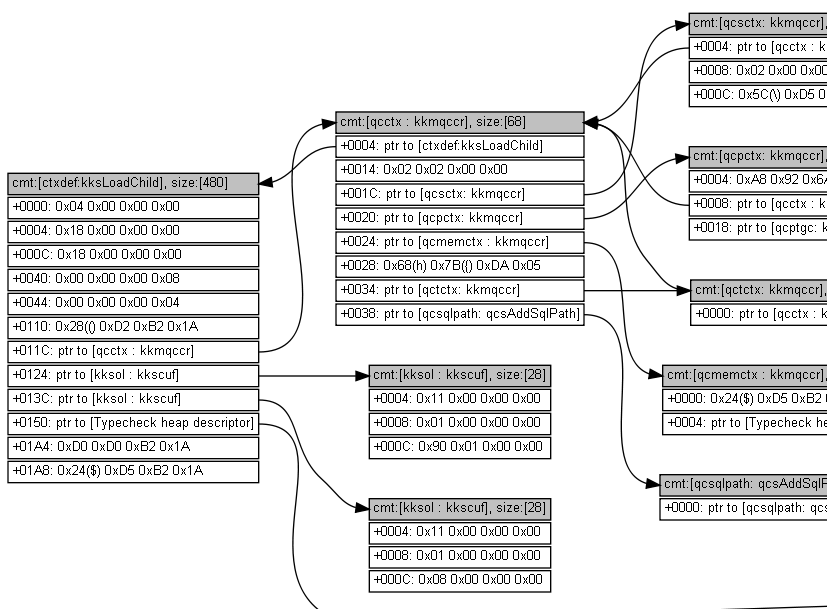
\includegraphics[scale=0.55]{advanced/450_more_ptrs/oracle2_crop.png}
\end{figure}

Bigger pictures:
\href{https://raw.githubusercontent.com/DennisYurichev/RE-for-beginners/master/advanced/450_more_ptrs/oracle1.png}{1},
\href{https://raw.githubusercontent.com/DennisYurichev/RE-for-beginners/master/advanced/450_more_ptrs/oracle2.png}{2}.

This is quite impressive, given the fact that I had no information about data types of all these structures.
But I could get some information from it.

\subsubsection{Now the garbage collector for C/C++: Boehm GC}

\myindex{Garbage collector}
If you use a block allocated in memory, its address has to be present somewhere, as a pointer in some structure/array in another allocated block,
or in globally allocated structure, or in local variable in stack.
If there are no pointer to a block, you can call it "orphan", and it will be a reason of memory leak.

And this is what \ac{GC} does.
It scans all blocks (because it keep tabs on all blocks allocated) for pointers.
It's important to understand, that it has no idea of data types of all these structure fields in blocks---this is important, \ac{GC} has no information about types.
It just scans blocks for 32-bit of 64-bit words and see, if they could be a pointers to another block(s).
It also scans stack.
It treats allocated blocks and stack as arrays of words, some of which may be pointers.
And if it found a block allocated, which is "orphaned", i.e., there are no pointer(s) to it from another block(s) or stack, this block considered unneeded, to be freed.
Scanning process takes time, and this is what for \ac{GC}s are criticized.

\myindex{Boehm garbage collector}
Also, \ac{GC} like Boehm GC\footnote{\url{https://www.hboehm.info/gc/}} (for pure C) has function like \verb|GC_malloc_atomic()|---using it, you declare that the block allocated
using this function will never contain any pointer(s) to other block(s).
Maybe this could be a text string, or other type of data.
(Indeed, \verb|GC_strdup()| calls \verb|GC_malloc_atomic()|.)
\ac{GC} will not scan it.

% Even more: if \ac{GC}'s memory allocator thinks it can find a better place for a block, it can \emph{move} it to another place, and then fix (rewrite) all addresses,
% pointing to it, in all other blocks and in stack.

